\documentclass[a4paper, 11 pt, conference]{article}  % Comment this line out
                                                          % if you need a4paper

% The following packages can be found on http:\\www.ctan.org
\usepackage{fontspec}
\usepackage{graphics} % for pdf, bitmapped graphics files
\usepackage{epsfig} % for postscript graphics files
\usepackage{mathptmx} % assumes new font selection scheme installed
\usepackage{times} % assumes new font selection scheme installed
\usepackage{amsmath} % assumes amsmath package installed
\usepackage{amssymb}  % assumes amsmath package installed
\usepackage{url}
\usepackage{inputenc}

\setromanfont{FreeSerif}

\title{\textbf{Practical New Developments on BREACH}}

\author{
        Dimitris Karakostas\footnotemark[1]\\
        National Technical University of Athens\\
        dimit.karakostas@gmail.com\\
        \and
        Dionysis Zindros\thanks{Research supported by ERC project CODAMODA, project \#259152.}\\
        University of Athens\\
        dionyziz@gmail.com\\
}

\date{}
\pagenumbering{arabic}

%%%%%%%%%%%%%%%%%%%%%%%%%%%%%%%%%%%%%%%%%%%%%%%%%%%%%%%%%%%%%%%%%%%%%%%%%%%%%%%%

\begin{document}

\maketitle
\thispagestyle{plain}
\pagestyle{plain}

%%%%%%%%%%%%%%%%%%%%%%%%%%%%%%%%%%%%%%%%%%%%%%%%%%%%%%%%%%%%%%%%%%%%%%%%%%%%%%%%

\begin{abstract}

We propose new methods to practically extend the BREACH attack against the most
commonly used ciphers. We describe a command-and-control technique to
exploit plain HTTP connections in order to perform the attack in a persistent manner.
We also present new statistical methods that can be used to bypass noise induced by
the usage of block ciphers, as well as noise present in usual web applications. In that
direction, we developed a new framework, Rupture, to explore parallelization and
optimization techniques. Finally, we propose novel mitigation techniques that could
effectively eliminate this attack.

\end{abstract}

%%%%%%%%%%%%%%%%%%%%%%%%%%%%%%%%%%%%%%%%%%%%%%%%%%%%%%%%%%%%%%%%%%%%%%%%%%%%%%%%
\section{Introduction}

In 2012, side-channel compression attacks were first successfully used against
TLS in CRIME \cite{c1}. CRIME targeted HTTPS requests, but it was mitigated by
disabling compression at the TLS level \cite{c2}.

In 2013, BREACH \cite{c3} was the sensation of Black Hat USA, introducing an attack vector that
exploited compression on HTTP responses to compromise SSL connections. Specifically, it
used the characteristics of the DEFLATE algorithm \cite{c4}, the basis of most compression
applications today, to steal secrets from applications using stream ciphers.

Three years later, RC4 is considered unsafe \cite{c5} and most websites use the AES block cipher. Some
services, such as Facebook, also went on to incorporate mechanisms to prevent
BREACH \cite{c6}.
However, the fundamental aspects of BREACH are still not mitigated and popular websites,
including Facebook, continue support for vulnerable end-points.

Our work demonstrates that BREACH can evolve to attack major web applications, confirming
the fact that TLS traffic is still practically vulnerable.

We incorporate statistical methods to bypass noise, induced either due to block ciphers or
random data included in the response plaintext. This allows us
to steal secrets that were not previously considered targets of BREACH, as long as the
targeted website offers a proper attack end-point. We describe two such end-points on
widely used applications, Facebook Chat and Gmail.

Over the course of our work we developed Rupture, an open source framework that enables BREACH
and similar web-based attacks. Development focused mainly on extensibility and scalability, resulting in a
fairly modular design, allowing for easy future analysis and experiments on different parts of the tool.

We conclude that all existing mitigation mechanisms are insufficient and can be
bypassed or are not practical. Finally, we propose novel mitigation mechanisms
that completely protect against such attacks.

%%%%%%%%%%%%%%%%%%%%%%%%%%%%%%%%%%%%%%%%%%%%%%%%%%%%%%%%%%%%%%%%%%%%%%%%%%%%%%%%

\section{Attack model}

\subsection{Attack assumptions}

The original BREACH paper described specific assumptions in order for the attack to be able
to work. In this work, we relax some of these assumptions.

Firstly, the target website should use HTTPS and compress the response plaintext.
gzip is the most commonly used compression implementation on the web,
although all
compression algorithms that use LZ77 \cite{c7} are sufficient.

It is important to mention that LZ77 uses a 32KB window, regarding the distance of the compressed literal.
Given that, the attacker needs to verify that the secret and the reflection are within that window, otherwise LZ77 will
not apply.

BREACH assumed that the target website uses stream ciphers and has zero noise.
However, block ciphers, especially AES, are the most commonly used encryption
ciphers today. We extend the attack on block ciphers and render the
vast majority of websites practically vulnerable to the attack.

The target website should also provide an end-point, where an arbitrary URL
parameter is reflected in the response along with the secret. This chosen
plaintext should be included in the same compression context as the secret. We
describe such end-points within Gmail and Facebook, although many other websites
expose similar vulnerabilities.

   \begin{figure}[thpb]
      \centering
      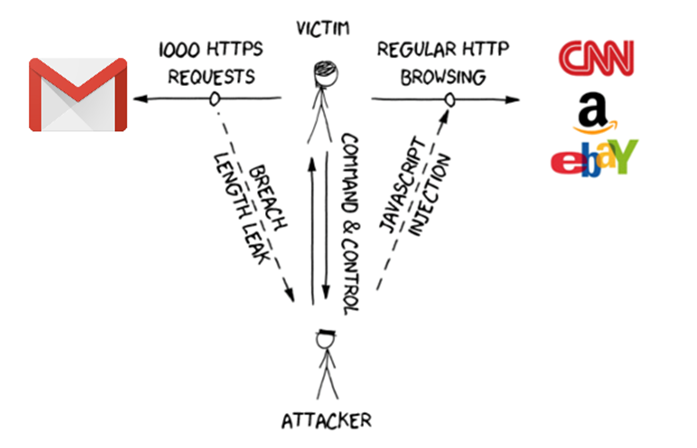
\includegraphics[width=0.9\textwidth]{figures/attack_model.png}
      \caption{Attack model}
   \end{figure}

\subsection{BREACH attack anatomy}

The first step is to gain control of the victim's network.
The attacker is able to inject code to the
victim's machine for execution. This code can issue adaptive requests to
the target service.

Our injector injects the client code in all unauthenticated HTTP responses that
the victim receives. This Javascript code is then executed by the victim's
browser in the context of the respective domain name.

The script issues multiple requests to the target website, which are sniffed and analyzed.

The client script runs in a different context from the
target website. Thus, it is subject to same-origin policy \cite{c8} and cannot read the
plaintext or encrypted responses. However, the encrypted requests and responses
are available to the sniffer through direct network access. By comparing the
encrypted lengths, information about the corresponding
plaintext length relationships can be deduced.

Each request contains chosen data, such as a URL parameter, that is reflected in the
response. As these requests are made from the victim's browser, they contain
authentication cookies which authenticate the user to the target service.
This results in the
response body containing the secret, so both the reflection and the secret will be
compressed and encrypted together.

A successful attack completely decrypts a portion of the plaintext. The portion
of the plaintext which the attack tries to decrypt is the secret. That portion
is identified through an initially known prefix which distinguishes it from
other secrets. Each byte of the
secret can be drawn from a given alphabet, the secret's alphabet.

At each stage of the attack, a prefix of the secret is known, because that
portion of the secret has already been successfully decrypted. The prefix
decrypted grows until the whole secret becomes known, at which stage the attack
is completed. Due to length leak, compressed plaintext
that contains the correct candidate will be shorter and so will the encrypted ciphertext.

   \begin{figure}[thpb]
      \centering
      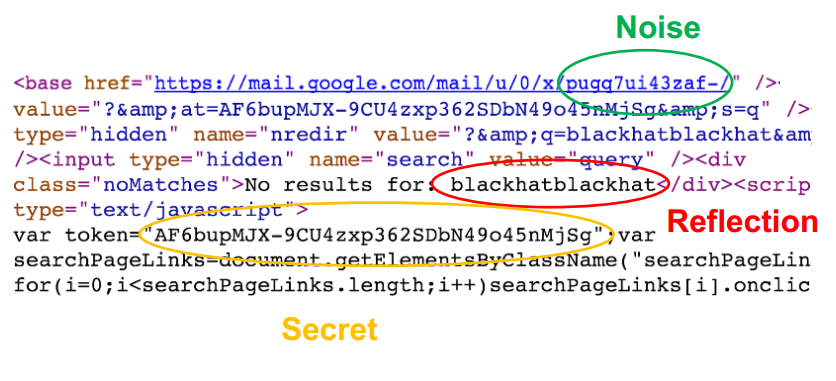
\includegraphics[width=1\textwidth]{figures/reflection.png}
      \caption{Response with reflection and noise}
   \end{figure}

\subsection{Alternative secrets}

The original BREACH attack targeted CSRF tokens and proposed mitigation methods based on this target.
In fact every part of the compressed plaintext is a possible secret. For
example, this could include private messages, e-mail communication and financial records.

%%%%%%%%%%%%%%%%%%%%%%%%%%%%%%%%%%%%%%%%%%%%%%%%%%%%%%%%%%%%%%%%%%%%%%%%%%%%%%%%

\section{Statistical methods}

\subsection{Block alignment}

Block ciphers provide a greater challenge compared to stream ciphers, when it
comes to telling length apart, since stream ciphers provide better granularity. That
is because block ciphers round length to $\lambda$-bits, where $\lambda$ is the block size,
by adding padding.

In order to bypass this, it is possible to introduce artificial noise, which will force the creation of
additional blocks, if necessary. Theoretically, it would be enough to issue
$16\times$ more requests
to achieve block alignment. At this point, the correct candidate would result in one less
block, which in turn would provide a measurable length difference. Block
alignment techniques have already been explored in the literature \cite{c9}.

However, introduction of artificial noise is actually tricky. Firstly, noise should be carefully constructed
to avoid being compressed with itself. Secondly, each added symbol will alter the Huffman coding in a
different way, since the plaintext's symbol frequency distribution will be altered. Even if the noise
includes symbols that do not appear in the rest of the plaintext, the Huffman tree will be expanded and,
consequently, the length of the compressed text will increase, in a manner that cannot always be
predicted.

\subsection{Noisy end-points}

In order to bypass noise, it should be enough to enforce statistical methods.
For that matter, it is possible to issue multiple requests per candidate alphabet symbol
and calculate the mean response length.

Given uniform noise with maximum compressed length $m$, the attack is expected to work in $O(n|\Sigma|\sqrt{m})$, where
$|\Sigma|$ is the length of the alphabet and $n$ is the length of the secret. Due to the Law of Large Numbers, length
converges to correct results.

%%%%%%%%%%%%%%%%%%%%%%%%%%%%%%%%%%%%%%%%%%%%%%%%%%%%%%%%%%%%%%%%%%%%%%%%%%%%%%%%

\section{Optimization techniques}

\subsection{Divide and conquer}

Up to this point, the characters of the alphabet were tested sequentially.
However, it is possible to use parallelization, that could effectively reduce the attack's time.

The idea behind this method is based on
\texttt{divide-and-conquer}. Specifically, instead of testing one
character at a time, concatenated with the known prefix, we split the
known alphabet into two candidate alphabet subsets which are tried
independently.

   \begin{figure}[thpb]
      \centering
      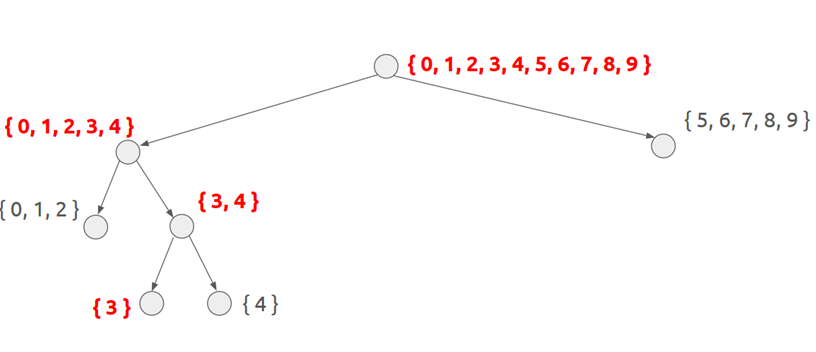
\includegraphics[width=0.9\textwidth]{figures/divide_and_conquer.png}
      \caption{Divide and Conquer}
   \end{figure}

The attack initially assumes the next unknown byte of the secret can come from
the secret's alphabet, but drills down and rejects alphabet symbols until
only one candidate symbol remains. At each stage of the attack for one byte of
the secret, there is a certain known alphabet which the next byte can take. This
known alphabet is a subset of the secret's alphabet.

Using this method, at each step of the attack two different requests are made.
The first corresponds to the top half of the alphabet and the second to the
bottom half.

This method reduces the time of the attack from
\begin{math}O(|\Sigma|)\end{math} to \begin{math}O(log|\Sigma|)\end{math},
which for example results in a $6\times$ speedup, given a candidate alphabet of 64 symbols.

\subsection{Request soup}

A problem with encrypted responses is the fact that it is not possible to safely
determine which packet corresponds to which request, when requests are pipelined
by the browser. That way if the attacker was to issue
requests sequentially, they would have to ensure all response packets for each request
have arrived, before issuing the next one.

However, it is possible to avoid this delay, by making samplesets, each one containing multiple
requests for a specific symbol. For each sampleset, responses would then come pipelined and it
would not be possible to tell them apart. However, the total length of the capture can still be
measured and divided by the known amount of requests that the sampleset
contains. This would be enough to calculate the desired mean length.

This method offers a speedup of up to $5\times$, considering a 200
ms delay and a 40 ms round trip time.

\subsection{Browser parallelization}

Browsers allow in general up to 6 parallel HTTP requests, although this may differ depending
on the browser application and release. This allows issuing multiple parallel requests and
collecting samples at the same time, giving the attack a $6\times$ speedup.

Each parallel request cannot adapt based on previous results.
However, we need to collect multiple samples per candidate to perform
statistical analysis and extract the mean. These samples pertain to the same
candidate and can be collected non-adaptively.

%%%%%%%%%%%%%%%%%%%%%%%%%%%%%%%%%%%%%%%%%%%%%%%%%%%%%%%%%%%%%%%%%%%%%%%%%%%%%%%%

\section{Vulnerable end-points}

We present two case studies where our findings apply, Gmail and Facebook Chat.
Both these services use AES and expose noisy end-points.

\subsection{Gmail}

Gmail uses an authentication token, which consists of random digits, letters
and dashes, generated every time the user logs into the account. The fact that
it does not change very often is
convenient because it allows the attacker to collect multiple samples for this
secret.

It also provides a mobile search functionality,
\url{https://mail.google.com/mail/u/0/x/?s=q\&q="search_string"},
that uses POST. However, GET still works, returning an error page that contains the authentication
token and reflects the GET parameter. This covers our reflection assumption.

The noise in this mobile end-point consists only of a randomly generated token.
This small amount of noise allows us to complete  the attack faster.

Attack bootstrapping is also trivial in this case, since all authentication tokens, regardless of login or
account, contain a fixed prefix, specifically "AF6bup".

\subsection{Facebook Chat}

Facebook has launched a mechanism to specifically prevent BREACH against its CSRF tokens.

However, it is a good case study to illustrate that there are more secrets in
addition to CSRF tokens. It provides a mobile version, Touch, that allows search on messages via GET, using
the following URL \url{https://touch.facebook.com/messages?q="search_string"}. This search query is reflected
in the search results page, along with the last message of the 5 latest conversations, regardless
of the search results. Instead of stealing the user's CSRF token, we can
therefore steal one of these private messages.

At this point, it might be reasonable to separate secrets from user input, as
the original BREACH paper recommends. However, in this case this distinction is
not possible. In case the attacker does not have access to a reflection
mechanism via URL parameters, it is possible to issue the attack as follows.
First, the attacker befriends the victim on Facebook. Then, to execute the
attack, specially crafted private messages would be sent to the victim and be
compressed together with the other 4 target messages.

%%%%%%%%%%%%%%%%%%%%%%%%%%%%%%%%%%%%%%%%%%%%%%%%%%%%%%%%%%%%%%%%%%%%%%%%%%%%%%%%

\section{Rupture}

Rupture is a framework for conducting network attacks against web services. It
is focused on compression-attacks, but provides a generalized scalable system
for performing any attack on web services which requires a persistent
command-and-control channel as well as attack adapation.
Rupture is suitable for any network chosen-plaintext attack.

Rupture was designed because all the available attack means to conduct BREACH
before it were at the proof-of-concept level and
did not provide a productized robust system that can work in real conditions. As
researchers, we spent a lot of time building separate proof-of-concept
implementations of BREACH and invested a lot of time to mount attacks against
specific end-points. Our motivation was that it takes a lot of effort to conduct
such an attack without the appropriate tools.

With rupture, our aim was to make it easier to mount such attacks and provide
reasonable pre-configured defaults, targets, and attack strategies that can be
used in practice or modified to suit the need of new attacks. The framework is
designed specifically to allow for further investigations on both the practical
and theoretical side. On the practical side, our network sniffing and injection
components are modular and replaceable. On the theoretical side, our analysis
and strategy core is independent of data collection means, allowing theoretical
cryptographers to verify or reject statistical analysis hypotheses through
experimental adaptive sample collection.

   \begin{figure}[thpb]
      \centering
      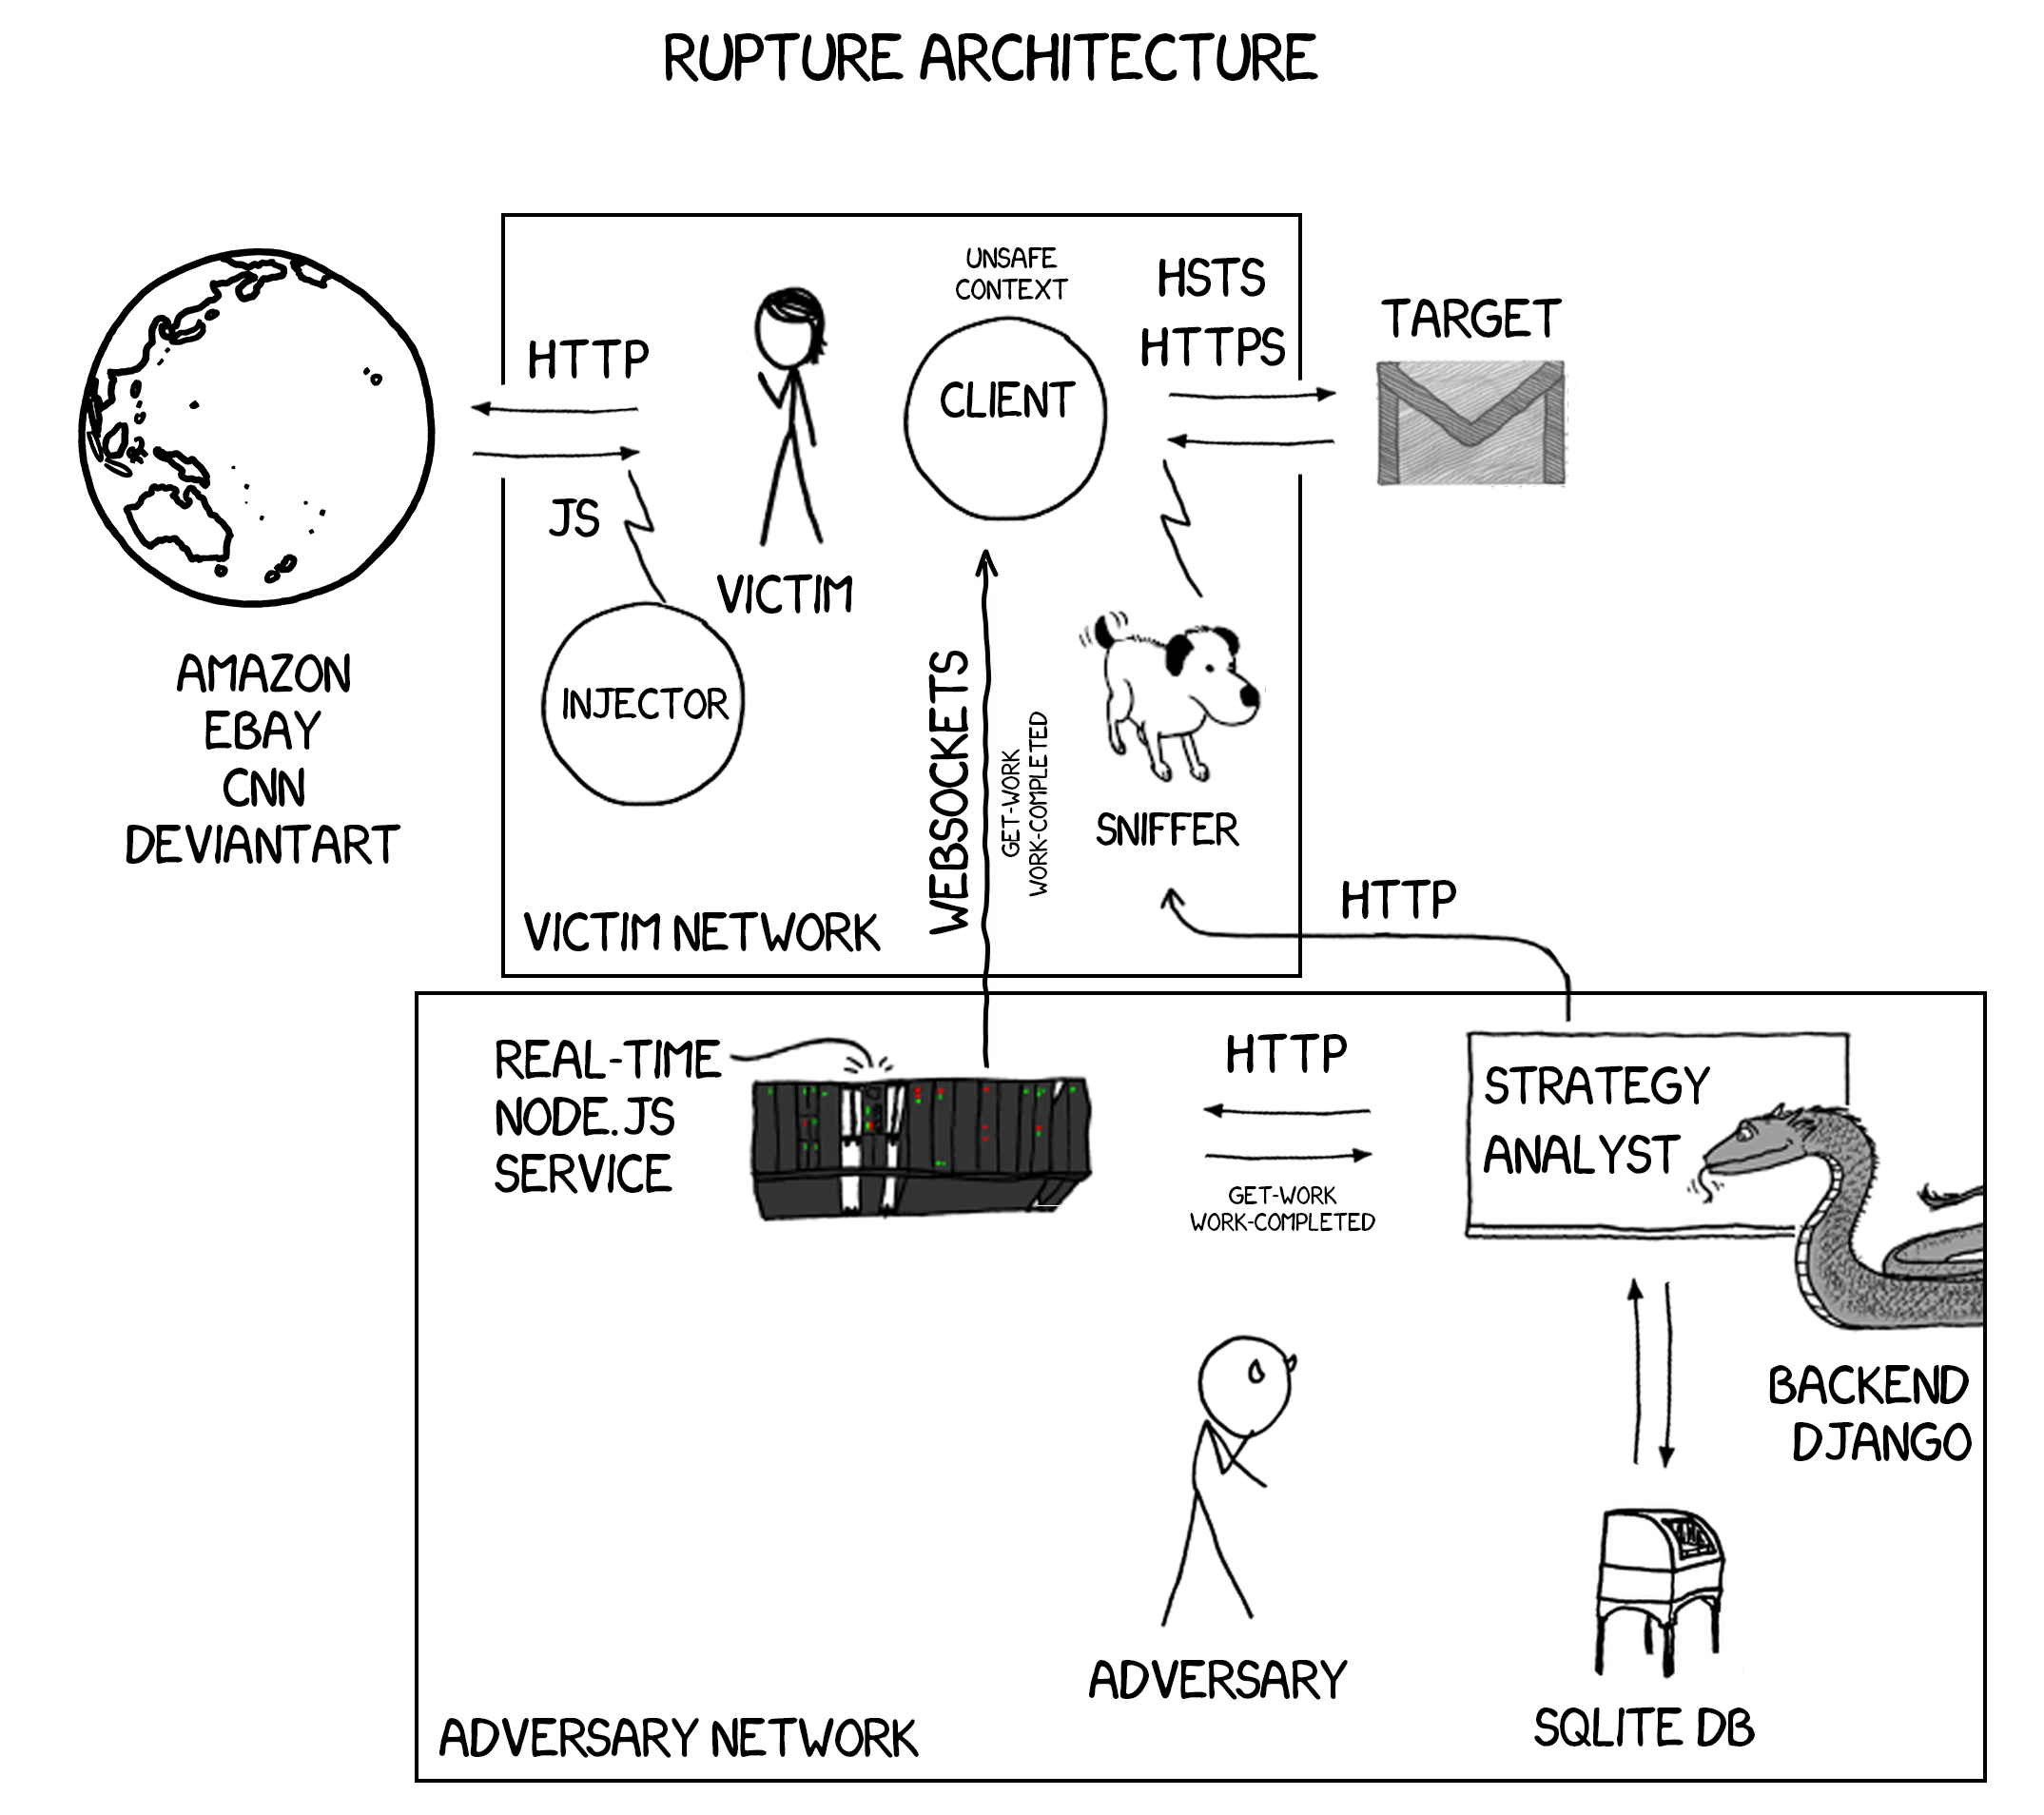
\includegraphics[width=0.7\textwidth]{figures/architecture.png}
      \caption{Rupture Architecture}
   \end{figure}

\subsection{Injector}
The injector component is responsible for injecting code to the victim's
computer for execution. We use Bettercap \cite{c10} to perform the HTTP
injection. The injection is performed by ARP spoofing the local network and
forwarding all traffic in a man-in-the-middle manner. It is simply a series of
shell scripts that use the appropriate bettercap modules to perform the attack.

Since all HTTP responses are infected, this provides for greatly increased
robustness.

The injector component needs to run on the victim network and as such is
light-weight and stateless. It can easily be deployed on a machine such as a
raspberry pi, and can be used for massive attacks. Multiple injectors can be
deployed to different networks, all controlled by the same central
command-and-control channel.

\subsection{Client}

The client contains minimal logic. It connects to the real-time service through
a command-and-control channel and registers itself there. Afterwards, it waits
for work instructions by the command-and-control channel, which it executes. The
client does not take any decisions or receive data about the progress of the
attack other than the work it is requested to do. This is intentional so as
to conceal the workings of the adversary analysis mechanisms from the victim
in case the victim attempts to reverse engineer what the adversary is doing.
Furthermore, it allows the system to be upgraded without having to deploy a
new client at the victim's network, which can be a difficult process.

As a regular user is browsing the Internet, multiple clients will be
injected in insecure pages and they will run under various contexts. All of
them will register and maintain an open connection through a
command-and-control channel with the real-time service. The real-time
service will enable one of them for this victim, while keeping the others
dormant. The one enabled will then receive work instructions to perform the
required requests. If the enabled client dies for whatever reason, such as a
closed tab, one of the rest of the clients will be waken up to take over the
attack.

\subsection{Real-time}

The real-time service is a service which awaits for work requests by clients. It
can handle multiple targets and victims. It receives command-and-control
connections from various clients which can live on different networks,
orchestrates them, and tells them which ones will remain dormant and which ones
will receive work, enabling one client per victim.

The real-time service is developed in node.js \cite{c11}. It maintains open web
socket command-and-control connections with clients and connects to the backend
service, facilitating the communication between the two.

\subsection{Sniffer}

The sniffer component is responsible for collecting data directly from the
victim's network. As the client issues chosen plaintext requests, the sniffer
collects the respective ciphertext requests and ciphertext responses as they
travel on the network. These encrypted data are then transmitted to the backend
for further analysis and decryption.

Our sniffer implementation runs on the same network as the victim. It is a
Python program which uses scapy \cite{c12} to collect network data.

The sniffer exposes an HTTP API which is utilized by the backend for controlling
when sniffing starts, when it is completed, and to retrieve the data that was
sniffed.

\subsection{Backend}

The backend is responsible for strategic decision taking, statistical analysis
of samples collected, adaptively advancing the attack, and storing persistent
data about the attacks in progress for future analysis.

The backend talks to the real-time service for pushing work out to clients. It
also speaks to the sniffer for data collection.

It is implemented in Python using the Django framework \cite{c13} and exposes a
RESTful API via HTTP to which the real-time services makes requests for work.

%%%%%%%%%%%%%%%%%%%%%%%%%%%%%%%%%%%%%%%%%%%%%%%%%%%%%%%%%%%%%%%%%%%%%%%%%%%%%%%%

\section{Mitigation}

\subsection{Failure of existing mechanisms}

The original BREACH paper proposed many mitigation mechanisms, some of which are
employed in real-world web applications.

Nevertheless, we have shown attack methodologies which defy these techniques.
Specifically:

\begin{itemize}
\item \textbf{Length hiding}: As mentioned in the BREACH paper, this method can
be bypassed using multiple requests. Indeed we have implemented the collection of
samplesets containing multiple samples in Rupture.
\item \textbf{Separating secrets from user input}: Contrary to the findings of
the original BREACH paper, we have illustrated through the Facebook case study
that secrets and user input can be inseparable.
\item \textbf{Disabling compression}: This mitigation is impractical in real-world systems.
\item \textbf{Masking secrets}: This method requires doubling the size of the
masked secret, which would be impractical for systems that offer many secrets,
such as social networks.
\item \textbf{Request rate-limiting}: This mitigation simply slows down the
attack and does not prevent it.
\end{itemize}

\subsection{First-party cookies}

The feasibility of the attack lies on the fact that the attacker can utilize the
target service as a compression oracle and retrieve encrypted compressed secrets
along with chosen plaintext data.

This is possible due to the fact that authentication cookies are included in
cross-origin requests. However, this inclusion is completely unnecessary for
most web applications. The ability to mark cookies as first-party only will
eliminate the existence of the oracle.

The first-party cookies proposal \cite{c14} describes such a mechanism, with the
purpose of avoiding CSRF attacks. Interestingly, the same mechanism can be used
to defend against compression side-channel attacks and eliminates the
possibility completely.

This proposal is still in draft stage and has not been implemented in any
browser. We urge browser vendors to adopt it immediately and web service authors
to opt-in.

%%%%%%%%%%%%%%%%%%%%%%%%%%%%%%%%%%%%%%%%%%%%%%%%%%%%%%%%%%%%%%%%%%%%%%%%%%%%%%%%

\section{Future work}

Further statistical analysis could probably result in better results. Given that
noise is a random variable, assuming the attacker has knowledge of its
properties, it would be useful to investigate how other aspects of the
distribution, such as higher moments, can be used in the analysis.

The attack framework assumes a target service to be attacked. Typically this
target service is a web service which uses TLS. Specifically, we are targeting
services that provide HTTPS end-points. However, this assumption can be relaxed
and attacks against other similar protocols are possible. Any protocol that
exchanges encrypted data on the network and for which a theoretical attack
exists can in principle be attacked using Rupture. We designed Rupture to be a
good playground for experimentation for such new attacks. Examples of other
encrypted protocols for which attacks can be tested include SMTP and XMPP.

This attack requires the victim has Javascript enabled. It is worthy exploring
whether the attack is still possible when Javascipt is disabled.

%%%%%%%%%%%%%%%%%%%%%%%%%%%%%%%%%%%%%%%%%%%%%%%%%%%%%%%%%%%%%%%%%%%%%%%%%%%%%%%%

\section{Acknowledgments}

This research was conducted at the Cryptography \& Security lab at the University of Athens
and the National Technical University of Athens.

We would like to thank Eva Sarafianou for her help in developing Rupture and
Angelo Prado, of the original BREACH team, for his continued support.

%%%%%%%%%%%%%%%%%%%%%%%%%%%%%%%%%%%%%%%%%%%%%%%%%%%%%%%%%%%%%%%%%%%%%%%%%%%%%%%%

\begin{thebibliography}{99}

\bibitem{c1} J. Rizzo, T. Duong: The CRIME attack, Ekoparty, 2012.

\bibitem{c2} [online] URL: \url{https://en.wikipedia.org/wiki/CRIME#Mitigation} [cited March 2016]

\bibitem{c3} Y. Gluck, N. Harris, A. Prado, BREACH: Reviving the CRIME attack,
Black Hat USA, 2013.

\bibitem{c4} [online] URL: \url{https://en.wikipedia.org/wiki/DEFLATE} [cited March 2016]

\bibitem{c5} A.Popov, Prohibiting RC4 Cipher Suites, RFC 7465, 2015.

\bibitem{c6} [online] URL: \url{https://www.facebook.com/notes/protect-the-graph/preventing-a-breach-attack/1455331811373632} [cited March 2016]

\bibitem{c7} J. Ziv, A. Lempel, A universal algorithm for sequential data
compression, Information Theory, IEEE Transactions, vol. 23, 1977.

\bibitem{c8} [online] URL: \url{https://en.wikipedia.org/wiki/Same-origin_policy} [cited March 2016]

\bibitem{c9} B. Moller, T. Duong, K. Kotowicz, This POODLE Bites: Exploiting the SSL 3.0 Fallback, September 2014.

\bibitem{c10} [online] URL: \url{https://www.bettercap.org/} [cited March 2016]

\bibitem{c11} [online] URL: \url{https://nodejs.org/en/} [cited March 2016]

\bibitem{c12} [online] URL: \url{http://www.secdev.org/projects/scapy/} [cited March 2016]

\bibitem{c13} [online] URL: \url{https://www.djangoproject.com/} [cited March 2016]

\bibitem{c14} M. West, First-Party-Only Cookies, RFC Internet-Draft, 2015.

\end{thebibliography}

\end{document}
